% !TeX program = xelatex
% Presentación de avance IPD-438: replicación de FAST-LoRa
% Compilar: latexmk -xelatex presentacion_avance.tex
\documentclass[aspectratio=169,11pt]{beamer}

\usefonttheme{professionalfonts}
\usepackage{fontspec}
\usepackage{unicode-math}
\setsansfont{Inter}[
  BoldFont       = {Inter SemiBold},
  ItalicFont     = {Inter Italic},
  BoldItalicFont = {Inter SemiBold Italic}]
\setmainfont{Inter}[
  BoldFont       = {Inter SemiBold},
  ItalicFont     = {Inter Italic},
  BoldItalicFont = {Inter SemiBold Italic}]
\setmathfont{Noto Sans Math}
\usepackage[spanish,es-noshorthands]{babel}
\usepackage{booktabs}
\usepackage{tikz}
\usepackage{pgfplots}
\pgfplotsset{compat=1.18,/pgf/number format/use comma,/pgf/number format/1000 sep={}}
\usetikzlibrary{arrows.meta,positioning,calc}

% ---------- Colores: un acento frío y uno cálido para lo que "no calza" ----------
\definecolor{ink}{HTML}{1F2933}
\definecolor{muted}{HTML}{66727F}
\definecolor{accent}{HTML}{0E6F7C}
\definecolor{warm}{HTML}{C2511A}
\definecolor{soft}{HTML}{EEF3F5}
\definecolor{softwarm}{HTML}{FBEEE6}

% ---------- Plantilla sobria: sin logos, sin fondos, sin barras ----------
\setbeamertemplate{navigation symbols}{}
\setbeamercolor{normal text}{fg=ink,bg=white}
\setbeamercolor{structure}{fg=accent}
\setbeamercolor{frametitle}{fg=ink}
\setbeamerfont{frametitle}{size=\Large,series=\bfseries}
\setbeamersize{text margin left=10mm,text margin right=10mm}
\setbeamertemplate{itemize items}{\textcolor{accent}{\raisebox{0.1ex}{$\bullet$}}}
\setlength{\leftmargini}{1.1em}

% Indicador de etapa (puntuación visual), anclado dentro del margen derecho
\def\etapa{0}
\newcommand{\crumb}[2]{\ifnum\etapa=#1\textcolor{accent}{\bfseries #2}\else\textcolor{muted!55}{#2}\fi}
\setbeamertemplate{headline}{%
  \ifnum\etapa>0
    \begin{tikzpicture}[remember picture,overlay]
      \node[anchor=north east,inner sep=0pt,font=\scriptsize]
        at ([xshift=-10mm,yshift=-4.5mm]current page.north east)
        {\crumb{1}{Problema}\hspace{3.5mm}\crumb{2}{Conceptos}\hspace{3.5mm}\crumb{3}{Estado del arte}\hspace{3.5mm}\crumb{4}{Objetivo}};
    \end{tikzpicture}%
  \fi
  \vskip7.5mm}
\setbeamertemplate{frametitle}{%
  \usebeamerfont{frametitle}\usebeamercolor[fg]{frametitle}%
  \parbox{\linewidth}{\raggedright\insertframetitle}\par\vskip1.5mm}
\setbeamertemplate{footline}{%
  \hfill{\scriptsize\textcolor{muted}{\insertframenumber}}\hspace{7mm}\vspace{3.5mm}}

% Fuente al pie, abajo a la izquierda
\newcommand{\fuente}[1]{%
  \begin{tikzpicture}[remember picture,overlay]
    \node[anchor=south west,font=\scriptsize,text=muted,align=left,text width=13.2cm,inner sep=0pt]
      at ([xshift=10mm,yshift=3.5mm]current page.south west) {#1};
  \end{tikzpicture}}

% Número en círculo: reemplaza al puntero láser ("miren el 2")
\newcommand{\num}[2][accent]{%
  \tikz[baseline=(n.base)]\node[circle,fill=#1,text=white,font=\scriptsize\bfseries,
    inner sep=0pt,minimum size=4.2mm](n){#2};}

% Iconos simples
\tikzset{
  gw/.pic={
    \draw[line width=1.1pt,ink] (-0.24,0) -- (0,0.8) -- (0.24,0);
    \draw[line width=0.8pt,ink] (-0.14,0.33) -- (0.14,0.33);
    \fill[ink] (0,0.85) circle (0.06);
    \draw[line width=0.8pt,accent] (0,0.85) ++(-45:0.22) arc (-45:45:0.22);
    \draw[line width=0.8pt,accent] (0,0.85) ++(135:0.22) arc (135:225:0.22);},
  server/.pic={
    \foreach \k in {0,1,2}{
      \draw[ink,fill=white,rounded corners=1pt,line width=0.8pt]
        (-0.38,0.26*\k) rectangle (0.38,0.26*\k+0.2);
      \fill[accent] (0.25,0.26*\k+0.1) circle (0.035);}},
  sensor/.pic={
    \draw[ink,fill=white,rounded corners=1.5pt,line width=0.8pt]
      (-0.17,-0.13) rectangle (0.17,0.13);
    \fill[accent] (0,0) circle (0.05);},
  caja/.style={draw=accent,line width=0.9pt,rounded corners=2mm,fill=soft,
    align=center,inner sep=2mm,font=\small},
  flecha/.style={-{Stealth[length=2.6mm]},line width=1pt,muted},
  tarjeta/.style={fill=soft,rounded corners=2.5mm,align=left,inner sep=3mm,anchor=north west,font=\small},
}

\title{¿Calcular en vez de simular?}
\author{Matias Perez Nieto}

\begin{document}

% =====================================================================
% 1 · PORTADA (la promesa se dice en voz alta; queda escrita en la lámina 4)
% =====================================================================
\begin{frame}[plain]
  \begin{tikzpicture}[remember picture,overlay]
    \node[anchor=north west,align=left,text width=10.2cm,inner sep=0pt]
      at ([xshift=12mm,yshift=-17mm]current page.north west) {%
      {\fontsize{27}{31}\selectfont\bfseries ¿Calcular en vez\\de simular?}\\[5mm]
      {\large Replicación independiente de la validación de FAST-LoRa}\\[8mm]
      {\normalsize Matias Perez Nieto}\\[1mm]
      {\small\textcolor{muted}{IPD-438 · Presentación de avance · 27 de octubre de 2026}}};
    \node[anchor=south west,align=left,text width=13.6cm,font=\scriptsize,text=muted,inner sep=0pt]
      at ([xshift=12mm,yshift=6mm]current page.south west) {%
      Paper base: L.~Acosta-García, J.~Aznar-Poveda, F.~Margreiter, A.-J.~García-Sánchez, J.~García-Haro, T.~Fahringer,
      J.~Lorente López y J.-V.~Rodríguez, “FAST-LoRa: An efficient simulation framework for evaluating LoRaWAN networks
      and transmission parameter strategies”, \emph{IEEE Access}, vol.~14, pp.~33518--33533, 2026.};
    % Símbolo de la charla: la vuelta completa del reloj (5 min) contra una astilla (8 ms)
    \begin{scope}[shift={([xshift=-32mm,yshift=-37mm]current page.north east)}]
      \draw[line width=5pt,accent!20] (0,0) circle (15mm);
      \draw[line width=5pt,accent] (0,15mm) arc (90:-265:15mm);
      \draw[line width=5pt,warm] (0,15mm) arc (90:83:15mm);
      \node[font=\small,align=center] at (0,0) {\textcolor{accent}{\bfseries 5 min}\\[0.5mm]\textcolor{warm}{\bfseries 8 ms}};
    \end{scope}
  \end{tikzpicture}
\end{frame}

% =====================================================================
% 2 · PROBLEMA, con un ejemplo concreto primero
% =====================================================================
\def\etapa{1}
\begin{frame}{Diseñar una red LoRaWAN es elegir entre unas $10^{168}$ configuraciones}
  \vspace{3mm}
  \begin{columns}[T,onlytextwidth]
    \begin{column}{0.47\textwidth}
      \begin{tikzpicture}
        \fill[soft,rounded corners=3mm] (0,0) rectangle (6.2,2.6);
        \pgfmathsetseed{11}
        \foreach \i in {0,...,9}{\foreach \j in {0,...,9}{
          \pgfmathsetmacro\x{0.45+0.58*\i+0.15*rand}
          \pgfmathsetmacro\y{0.22+0.24*\j+0.05*rand}
          \fill[accent] (\x,\y) circle (0.5mm);}}
      \end{tikzpicture}\\[3mm]
      {\small\textcolor{muted}{100 sensores $\times$ 48 opciones cada uno (SF y potencia)}}\\[2mm]
      {\Large $48^{100}\approx\textcolor{accent}{10^{168}}$}
    \end{column}
    \begin{column}{0.47\textwidth}
      {\large ¿Cuánto cuesta evaluar \emph{una}?}\\[5mm]
      {\small\textcolor{muted}{FLoRa, simula paquete a paquete}}\\
      {\fontsize{22}{26}\selectfont\bfseries más de 5 min}\\[5mm]
      {\small\textcolor{muted}{FAST-LoRa, modelo analítico}}\\
      {\fontsize{22}{26}\selectfont\bfseries\textcolor{accent}{menos de 8 ms}}
    \end{column}
  \end{columns}
  \fuente{Tiempos para 200 nodos y 5 días simulados, Fig.~6 de [1]. SF de 7 a 12; potencia de 2 a 16 dBm en pasos de 2.}
\end{frame}

% =====================================================================
% 3 · INESTABILIDAD (McEnerney: "sin embargo")
% =====================================================================
\begin{frame}{FAST-LoRa promete rapidez sin perder exactitud, pero nadie lo ha verificado por fuera}
  \vspace{3mm}
  \begin{tikzpicture}[caja2/.style={rounded corners=3mm,text width=5.9cm,minimum height=3.3cm,inner sep=4mm,align=left,anchor=north west}]
    \node[caja2,fill=soft] (a) at (0,0) {%
      {\bfseries\textcolor{accent}{Lo que afirma el paper}}\\[2.5mm]
      Hasta 1000 veces más rápido\\[1.5mm]
      Error en la PDR: 0,94 puntos\\[1.5mm]
      Error en energía: 0,04 bits/mJ};
    \node[caja2,fill=softwarm] (b) at (7.1,0) {%
      {\bfseries\textcolor{warm}{Sin embargo}}\\[2.5mm]
      Lo validaron solo sus autores\\[1.5mm]
      contra un FLoRa que ellos modificaron,\\[1.5mm]
      con el ADR apagado\\[1.5mm]
      y con números que no calzan};
  \end{tikzpicture}\\[5mm]
  \centerline{\large Si el modelo se equivoca, también las redes diseñadas con él.}
  \fuente{[1] Acosta-García et al., 2026. PDR: fracción de paquetes que llegan. ADR: el servidor ajusta SF y potencia de cada nodo.}
\end{frame}

% =====================================================================
% 4 · PROMESA Y MAPA (3 puntos, después de la motivación)
% =====================================================================
\begin{frame}{Al terminar van a saber cuándo creerle a un simulador de 8 ms}
  \vspace{10mm}
  \begin{tikzpicture}[
      card/.style={draw=accent,line width=1pt,rounded corners=3mm,text width=3.6cm,
        minimum height=2.6cm,align=left,inner sep=3.5mm,anchor=north west},
      big/.style={font=\fontsize{24}{24}\selectfont\bfseries,text=accent}]
    \node[card] (a) at (0,0)    {{\bfseries Conceptos}\\[2mm]\small Por qué un paquete LoRa llega o se pierde};
    \node[card] (b) at (4.75,0) {{\bfseries Estado del arte}\\[2mm]\small Qué existe y qué encontré al leer con lupa};
    \node[card] (c) at (9.5,0)  {{\bfseries Objetivo}\\[2mm]\small Qué voy a reproducir y cómo sabré si coincide};
    \foreach \n/\t in {a/1,b/2,c/3}
      \node[big,anchor=south west] at ([xshift=0.5mm,yshift=0.5mm]\n.north west) {\t};
  \end{tikzpicture}
\end{frame}

% =====================================================================
% 5 · CONCEPTOS: LoRaWAN con un ejemplo
% =====================================================================
\def\etapa{2}
\begin{frame}{En LoRaWAN los sensores transmiten sin coordinarse y cualquier gateway puede escucharlos}
  \begin{center}
  \begin{tikzpicture}[x=1cm,y=0.85cm,lbl/.style={font=\footnotesize,align=left,anchor=north west,text=ink,inner sep=0pt}]
    \foreach \x/\y/\n in {0.4/2.5/s1,1.5/3.1/s2,0.8/1.6/s3,2.1/2.0/s4,1.2/0.6/s5,2.5/0.9/s6}
      \coordinate (\n) at (\x,\y);
    \coordinate (g1) at (6.2,2.3);
    \coordinate (g2) at (6.2,0.3);
    \coordinate (ns) at (11.4,1.3);
    \foreach \s/\g in {s1/g1,s2/g1,s3/g1,s5/g2,s6/g2}
      \draw[muted!60,dashed,line width=0.7pt] (\s) -- ([yshift=6mm]\g);
    \draw[accent,line width=1.4pt,dashed] (s4) -- ([yshift=6mm]g1);
    \draw[accent,line width=1.4pt,dashed] (s4) -- ([yshift=6mm]g2);
    \foreach \s in {s1,s2,s3,s5,s6} \pic at (\s) {sensor};
    \pic[scale=1.3] at (s4) {sensor};
    \pic at (g1) {gw};  \pic at (g2) {gw};
    \pic at (ns) {server};
    \draw[ink,line width=1pt] ([xshift=3mm,yshift=4mm]g1) -- ([xshift=-4.5mm,yshift=5mm]ns);
    \draw[ink,line width=1pt] ([xshift=3mm,yshift=4mm]g2) -- ([xshift=-4.5mm,yshift=2mm]ns);
    \node[font=\scriptsize,text=muted] at (8.7,1.62) {Internet (IP)};
    \node[font=\small,text=muted] at (1.4,3.75) {Sensores};
    \node[font=\small,text=muted] at (6.2,3.75) {Gateways};
    \node[font=\small,text=muted] at (11.4,3.75) {Servidor de red};
    \node at (2.15,2.6) {\num{1}};
    \node at (4.35,1.05) {\num{2}};
    \node at (11.4,2.55) {\num{3}};
    % leyenda en tres columnas de ancho fijo
    \node[lbl,text width=4.1cm] at (-0.2,-0.45) {\num{1}\ Transmite sin escuchar el canal (ALOHA puro)};
    \node[lbl,text width=4.1cm] at (4.6,-0.45)  {\num{2}\ El mismo paquete llega a dos gateways};
    \node[lbl,text width=4.1cm] at (9.3,-0.45)  {\num{3}\ Descarta duplicados y ajusta SF y potencia (ADR)};
  \end{tikzpicture}
  \end{center}
  \vspace{2mm}
  \centerline{\colorbox{soft}{\small\strut\ Ejemplo: un sensor de riego que envía 10 bytes cada 17 minutos, solo de subida\ }}
\end{frame}

% =====================================================================
% 6 · CONCEPTOS: spreading factor
% =====================================================================
\begin{frame}{El spreading factor (SF) cambia alcance por tiempo en el aire}
  \begin{columns}[c,onlytextwidth]
    \begin{column}{0.52\textwidth}
      \begin{tikzpicture}
        \begin{axis}[
            width=7.6cm,height=5.2cm,ybar,bar width=7mm,bar shift=0pt,
            ymin=0,ymax=1150,axis lines*=left,
            symbolic x coords={SF7,SF8,SF9,SF10,SF11,SF12},xtick=data,
            ylabel={tiempo en el aire (ms)},ylabel style={font=\small,text=muted},
            tick label style={font=\small},ytick={0,500,1000},
            nodes near coords,nodes near coords style={font=\scriptsize,text=ink},
            enlarge x limits=0.12]
          \addplot[fill=accent,draw=none] coordinates {(SF7,36) (SF8,72) (SF9,124) (SF10,248) (SF11,496)};
          \addplot[fill=warm,draw=none] coordinates {(SF12,991)};
        \end{axis}
      \end{tikzpicture}
    \end{column}
    \begin{column}{0.44\textwidth}
      {\large De SF7 a SF12:}\\[3mm]
      {\Large\textcolor{warm}{27 veces}} {\large más tiempo en el aire}\\[1mm]
      {\small\textcolor{muted}{más energía y más choques}}\\[7mm]
      {\large pero entiende señales}\\[1mm]
      {\Large\textcolor{accent}{100 veces}} {\large más débiles que el ruido}\\[1mm]
      {\small\textcolor{muted}{SNR mínima: $-20$~dB en SF12}}
    \end{column}
  \end{columns}
  \fuente{Ec.~(1) a (5) y Tabla~1 de [1], con $B=125$~kHz, CR 4/5 y payload de 10~B (el que usa el código de los autores).}
\end{frame}

% =====================================================================
% 7 · CONCEPTOS: se pierde si llega débil
% =====================================================================
\begin{frame}{Un paquete se pierde si llega débil…}
  \begin{center}
  \begin{tikzpicture}
    \begin{axis}[width=11cm,height=4.9cm,axis lines=left,ymin=0,ymax=0.13,
        xmin=-138,xmax=-108,ytick=\empty,xtick=\empty,
        xlabel={potencia recibida (dBm)},xlabel style={font=\small,text=muted},
        domain=-138:-108,samples=90,clip=false]
      \addplot[draw=none,fill=accent!25,domain=-127:-108] {exp(-(x+122)^2/(2*3.57^2))/(3.57*sqrt(2*pi))} \closedcycle;
      \addplot[draw=none,fill=warm!20,domain=-138:-127] {exp(-(x+122)^2/(2*3.57^2))/(3.57*sqrt(2*pi))} \closedcycle;
      \addplot[accent,line width=1.3pt] {exp(-(x+122)^2/(2*3.57^2))/(3.57*sqrt(2*pi))};
      \draw[warm,line width=1.3pt] (axis cs:-127,0) -- (axis cs:-127,0.125);
      \node[font=\small,text=warm,anchor=south] at (axis cs:-127,0.125) {sensibilidad};
      \node[font=\large,text=accent] at (axis cs:-118.5,0.045) {$\psi$ = llega};
      \node[font=\small,text=warm,anchor=east] at (axis cs:-128,0.035) {se pierde};
    \end{axis}
  \end{tikzpicture}
  \end{center}
  \vspace{1mm}
  \centerline{\normalsize La señal baja con la distancia y además varía al azar en cada paquete.}
  \fuente{Ec.~(7) y (8) de [1]: pérdida log-distancia con desvanecimiento gaussiano, $\sigma=3{,}57$~dB. La sensibilidad depende del SF.}
\end{frame}

% =====================================================================
% 8 · CONCEPTOS: o si choca con otro
% =====================================================================
\begin{frame}{…o si choca con otro paquete}
  \begin{center}
  \begin{tikzpicture}[x=1.3cm,y=1.1cm]
    \draw[muted,-{Stealth}] (0,0) -- (7,0) node[right,font=\small] {$t$};
    \fill[accent!30] (1.2,0.12) rectangle (2.9,0.7);
    \fill[warm!70] (2.2,0.12) rectangle (2.9,0.7);
    \fill[accent] (2.9,0.12) rectangle (6.4,0.7);
    \node[font=\small] at (1.7,0.41) {preámbulo};
    \node[font=\small,text=white] at (4.65,0.41) {paquete A};
    \fill[muted!50] (-0.2,0.95) rectangle (2.55,1.5);
    \node[font=\small] at (1.15,1.22) {paquete B};
    \draw[warm,line width=0.9pt,dashed] (2.2,-0.08) -- (2.2,1.65);
    \draw[warm,line width=0.9pt,dashed] (2.9,-0.08) -- (2.9,1.65);
    \node[font=\small,text=warm] at (2.55,1.9) {últimos 5 símbolos};
  \end{tikzpicture}
  \end{center}
  \vspace{1mm}
  \centerline{\normalsize A se pierde si B pisa esos símbolos y A no llega al menos 6~dB más fuerte.}
  \vspace{4mm}
  \centerline{\colorbox{soft}{\parbox{0.8\linewidth}{\centering\strut
    $\mathrm{PDR}=\textcolor{accent}{\psi}\cdot\textcolor{warm}{\zeta}$\\[1mm]
    {\small\textcolor{muted}{llega fuerte $\times$ no choca; con varios gateways basta que uno lo reciba}}\strut}}}
  \fuente{Ec.~(9) a (13) de [1]. Con SF distintos el umbral es negativo y casi siempre sobrevive (Tabla~3 de [1], Croce et al. 2018).}
\end{frame}

% =====================================================================
% 9 · CONCEPTOS: simular contra calcular (idea central)
% =====================================================================
\begin{frame}{FLoRa cuenta paquetes, FAST-LoRa calcula probabilidades}
  \vspace{2mm}
  \begin{columns}[T,onlytextwidth]
    \begin{column}{0.48\textwidth}
      {\bfseries FLoRa} {\small\textcolor{muted}{[2]}}\\[3mm]
      \begin{tikzpicture}[x=1cm,y=1cm]
        \pgfmathsetseed{3}
        \foreach \r/\lab in {0/ED3,1/ED2,2/ED1}{
          \node[font=\scriptsize,text=muted,anchor=east] at (-0.05,\r*0.45+0.18) {\lab};
          \foreach \k in {1,...,13}{
            \pgfmathsetmacro\x{0.45*\k+0.3*rand}
            \fill[accent] (\x,\r*0.45+0.06) rectangle ++(0.08,0.22);}}
        \draw[muted,-{Stealth}] (0,-0.05) -- (6.4,-0.05) node[below left,font=\scriptsize] {5 días simulados};
      \end{tikzpicture}\\[3mm]
      {\small Genera cada paquete y cuenta los que llegan}
    \end{column}
    \begin{column}{0.48\textwidth}
      {\bfseries\textcolor{accent}{FAST-LoRa}} {\small\textcolor{muted}{[1]}}\\[3mm]
      \begin{tikzpicture}[x=1cm,y=1cm]
        \foreach \r in {0,...,3}{\foreach \c in {0,...,3}{
          \draw[accent,fill=soft] (\c*0.6,\r*0.32) rectangle ++(0.54,0.26);}}
        \node[font=\scriptsize,text=muted,rotate=90] at (-0.3,0.62) {nodos};
        \node[font=\scriptsize,text=muted] at (1.17,1.48) {gateways};
        \draw[flecha] (2.6,0.62) -- (3.4,0.62);
        \node[font=\small,anchor=west] at (3.45,0.62) {PDR, energía};
      \end{tikzpicture}\\[3mm]
      {\small Evalúa $\psi$ y $\zeta$ para todos los nodos de una vez}
    \end{column}
  \end{columns}
  \vspace{7mm}
  \centerline{\colorbox{soft}{\strut\ Lanzar una moneda mil veces, o calcular que la probabilidad es $1/2$\ }}
\end{frame}

% =====================================================================
% 10 · ESTADO DEL ARTE: mapa
% =====================================================================
\def\etapa{3}
\begin{frame}{Las herramientas para LoRa van de una fórmula cerrada a una red real}
  \begin{center}
  \begin{tikzpicture}[x=1cm,y=0.9cm,
      pt/.style={circle,fill=muted,inner sep=0pt,minimum size=2.2mm},
      lab/.style={font=\scriptsize,align=left,anchor=west,text=ink,inner sep=1pt}]
    \draw[muted,-{Stealth}] (0,0) -- (13.2,0);
    \draw[muted,-{Stealth}] (0,0) -- (0,4.7);
    \node[font=\scriptsize,text=muted,rotate=90] at (-1.05,2.3) {costo de evaluar una red};
    \foreach \y/\t in {0.45/ms,1.55/s,2.75/min,3.95/horas}
      \node[font=\scriptsize,text=muted,anchor=east] at (-0.1,\y) {\t};
    \foreach \x/\t in {1.6/fórmula cerrada,4.9/modelo por nodo,8.4/paquete a paquete,11.8/red real}
      \node[font=\scriptsize,text=muted] at (\x,-0.3) {\t};
    \node[font=\scriptsize,text=muted,anchor=east] at (13.2,-0.62) {más detalle $\rightarrow$};
    \node[pt] (aloha) at (0.4,0.35) {};  \node[lab] at ([xshift=1mm]aloha.east) {ALOHA puro\\Abramson 1970};
    \node[pt] (geo)   at (1.8,1.0) {};   \node[lab] at ([xshift=1mm]geo.east) {geometría estocástica\\Georgiou y Raza 2017};
    \node[pt] (toro)  at (4.3,1.75) {};  \node[lab,anchor=east,align=right] at ([xshift=-1mm]toro.west) {modelo por dispositivo\\Toro-Betancur et al. 2021};
    \node[pt,fill=accent,minimum size=3.2mm] (fast) at (4.6,0.4) {};
      \node[lab,text=accent] at ([xshift=1.5mm]fast.east) {\bfseries FAST-LoRa 2026};
    \node[pt] (lsim)  at (7.3,2.2) {};   \node[lab] at ([xshift=1mm]lsim.east) {LoRaSim (Python)\\Bor et al. 2016};
    \node[pt] (ns3)   at (9.4,3.0) {};   \node[lab] at ([xshift=1mm]ns3.east) {ns-3 lorawan\\Magrin 2017\\Van den Abeele 2017};
    \node[pt,fill=warm,minimum size=3.2mm] (flora) at (8.6,3.95) {};
      \node[lab,text=warm,anchor=east] at ([xshift=-1.5mm]flora.west) {\bfseries FLoRa 2018 (OMNeT++)};
    \node[pt] (real)  at (10.9,4.4) {};  \node[lab] at ([xshift=1mm]real.east) {red física\\o LWN-Simulator};
    \draw[{Stealth}-{Stealth},line width=1pt,ink,dashed,shorten <=2.5mm,shorten >=2.5mm]
      (fast) -- node[pos=0.5,sloped,above,font=\scriptsize,inner sep=1.5pt] {lo que voy a comparar} (flora);
  \end{tikzpicture}
  \end{center}
  \fuente{Ubicación cualitativa. A octubre de 2026 FAST-LoRa tiene 4 citas, 3 del mismo grupo, y ninguna réplica independiente.}
\end{frame}

% =====================================================================
% 11 · ESTADO DEL ARTE: qué me llevo de cada lectura
% =====================================================================
\begin{frame}{Lo que me llevo de cada lectura}
  \vspace{4mm}
  \begin{tikzpicture}[t/.style={tarjeta,text width=3.75cm,minimum height=2.15cm}]
    \node[t] at (0,0)       {{\bfseries Bor et al. 2016} {\scriptsize\textcolor{muted}{[3]}}\\[1.5mm]De aquí salen los parámetros de propagación};
    \node[t] at (4.75,0)    {{\bfseries Croce et al. 2018} {\scriptsize\textcolor{muted}{[4]}}\\[1.5mm]Los SF no son del todo independientes entre sí};
    \node[t] at (9.5,0)     {{\bfseries Van den Abeele 2017} {\scriptsize\textcolor{muted}{[5]}}\\[1.5mm]ALOHA puro no basta: hay efecto captura};
    \node[t] at (0,-2.55)   {{\bfseries Toro-Betancur 2021} {\scriptsize\textcolor{muted}{[6]}}\\[1.5mm]El modelo de FAST-LoRa ya existía, vía Zhang 2023};
    \node[t] at (4.75,-2.55){{\bfseries Liando et al. 2019} {\scriptsize\textcolor{muted}{[8]}}\\[1.5mm]Consumo medido en hardware real};
    \node[t] at (9.5,-2.55) {{\bfseries Lima et al. 2024} {\scriptsize\textcolor{muted}{[9]}}\\[1.5mm]Otro entorno, otros parámetros};
  \end{tikzpicture}
\end{frame}

% =====================================================================
% 12 · ESTADO DEL ARTE: lectura crítica del paper (la sorpresa)
% =====================================================================
\begin{frame}{Leyendo el paper con lupa aparecen cuatro cabos sueltos}
  \vspace{4mm}
  \begin{tikzpicture}[t/.style={tarjeta,fill=softwarm,text width=5.95cm,minimum height=2.1cm}]
    \node[t] at (0,0)      {\num[warm]{1}\ {\bfseries Falta el tamaño del paquete}\\[2mm]No está en el paper; el código usa 10 bytes};
    \node[t] at (7.1,0)    {\num[warm]{2}\ {\bfseries Dos promedios mezclados}\\[2mm]0,040 promedia por nodo; 0,038 por tabla};
    \node[t] at (0,-2.5)   {\num[warm]{3}\ {\bfseries Más rápido de lo que dice}\\[2mm]Sus tiempos dan unas $10^4$ veces, no $10^3$};
    \node[t] at (7.1,-2.5) {\num[warm]{4}\ {\bfseries Ecuación (11)}\\[2mm]Usa $2\sigma$ donde corresponde $\sqrt{2}\,\sigma$};
  \end{tikzpicture}
  \fuente{Cálculos propios con las Tablas~6 y 7, la Fig.~6 y la ec.~(11) de [1]. Detalle en las láminas de respaldo.}
\end{frame}

% =====================================================================
% 13 · ESTADO DEL ARTE: lo que muestra el código de los autores
% =====================================================================
\begin{frame}{El código muestra diferencias que el paper no menciona}
  \vspace{2mm}
  {\small\textcolor{muted}{Los experimentos están en otro repositorio del autor, no en el que cita el paper.}}\\[4mm]
  \renewcommand{\arraystretch}{1.55}
  \begin{tabular}{@{}p{5.6cm}p{3.6cm}p{3.6cm}@{}}
    \toprule
    & \textcolor{accent}{\bfseries FAST-LoRa} & \textcolor{muted}{\bfseries FLoRa} \\ \midrule
    Tiempo en el aire con SF12 & 0,99~s & \textcolor{warm}{1,42~s} \\
    Umbral entre paquetes del mismo SF & 6~dB & \textcolor{warm}{1~dB} \\
    Matriz de umbrales & \textcolor{warm}{al revés} & correcta \\
    Código del ADR & \textcolor{warm}{falla} & apagado \\
    \bottomrule
  \end{tabular}
  \fuente{Revisión propia de github.com/jaznrp/FastLoRa, jaznrp/MultiAgent-MARLTC y florasim/flora (octubre de 2026). Lista completa en el respaldo.}
\end{frame}

% =====================================================================
% 14 · OBJETIVO DEL SEMESTRE
% =====================================================================
\def\etapa{4}
\begin{frame}{Objetivo: repetir la validación por mi cuenta y medir si el error se mantiene}
  \vspace{4mm}
  \begin{center}
  \begin{tikzpicture}[
      b/.style={caja,minimum height=1.1cm,text width=2.0cm},
      bw/.style={caja,draw=warm,fill=softwarm,minimum height=1.1cm,text width=2.0cm}]
    \node[b] (topo) at (0,0) {Misma\\topología};
    \node[b] (flora) at (3.0,0.75)  {FLoRa};
    \node[b] (fast)  at (3.0,-0.75) {FAST-LoRa};
    \node[b] (met)   at (5.8,0)    {PDR y energía\\por nodo};
    \node[b] (err)   at (8.6,0)    {Error entre\\ambos};
    \node[bw] (cmp)  at (11.4,0)   {¿Igual que\\el paper?};
    \draw[flecha] (topo.east) -- (flora.west);
    \draw[flecha] (topo.east) -- (fast.west);
    \draw[flecha] (flora.east) -- (met.west);
    \draw[flecha] (fast.east) -- (met.west);
    \draw[flecha] (met) -- (err);
    \draw[flecha] (err) -- (cmp);
  \end{tikzpicture}
  \end{center}
  \vspace{6mm}
  {\normalsize\textcolor{accent}{Éxito}, fijado antes de simular: mismas tendencias y error del mismo orden que el paper.}\\[3mm]
  {\normalsize\textcolor{accent}{Alcance}: el del paper. Si queda tiempo, repetir con el ADR encendido.}
\end{frame}

% =====================================================================
% 15 · RESULTADO A REPRODUCIR
% =====================================================================
\begin{frame}{En la presentación final mostraré esta figura y esta tabla, hechas por mí}
  \vspace{2mm}
  \begin{columns}[T,onlytextwidth]
    \begin{column}{0.45\textwidth}
      \num{1}\ {\small\bfseries Un nodo y un gateway}\\[1mm]
      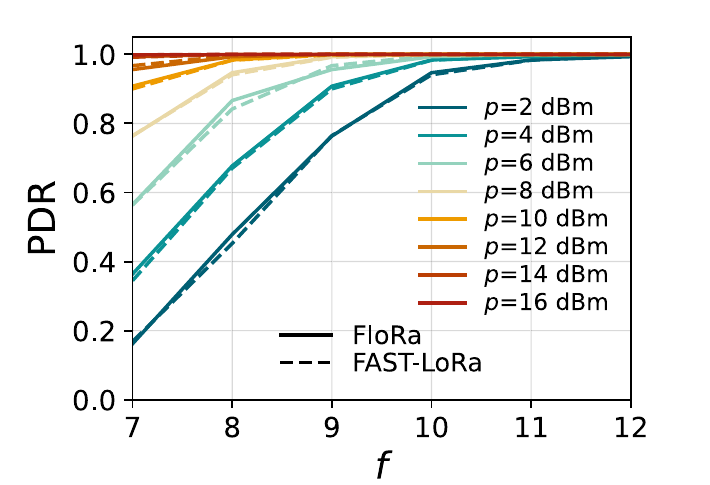
\includegraphics[width=0.85\linewidth]{figs/paper_fig3c.png}\\[-1mm]
      {\scriptsize\textcolor{muted}{PDR contra SF a 50 m (Fig.~3c de [1]). Continua: FLoRa; segmentada: FAST-LoRa.}}
    \end{column}
    \begin{column}{0.51\textwidth}
      \num{2}\ {\small\bfseries Redes densas: error en la PDR ($\times10^{-2}$)}\\[3mm]
      {\small
      \renewcommand{\arraystretch}{1.25}
      \begin{tabular}{@{}r cccc@{}}
        & \multicolumn{4}{c}{\textcolor{muted}{gateways}}\\
        \textcolor{muted}{nodos} & 1 & 2 & 3 & 4 \\ \midrule
        10  & 0,670 & 0,960 & 1,067 & 0,765 \\
        50  & 0,718 & 0,671 & 0,852 & 0,857 \\
        100 & 0,645 & 0,759 & 0,820 & 0,935 \\
        500 & 0,868 & 1,040 & 1,002 & \textcolor{warm}{\bfseries 1,044} \\ \bottomrule
      \end{tabular}}\\[2mm]
      {\scriptsize\textcolor{muted}{Tabla~6 de [1]. Promedio por nodo: \textcolor{accent}{0,940}.}}\\[4mm]
      \num{3}\ {\small\bfseries Tiempo de cómputo} {\scriptsize\textcolor{muted}{(Fig.~6 de [1])}}
    \end{column}
  \end{columns}
\end{frame}

% =====================================================================
% 16 · PLAN (se puede saltar si falta tiempo)
% =====================================================================
\begin{frame}{Plan hasta la presentación final}
  \vspace{10mm}
  \begin{tikzpicture}[x=1cm,y=1cm,
      hito/.style={circle,fill=accent,minimum size=3mm,inner sep=0pt},
      txt/.style={font=\small,align=left,anchor=north west,text width=3.0cm}]
    \draw[muted!50,line width=2pt] (0,0) -- (13.9,0);
    \node[hito,fill=warm,minimum size=4mm] at (0.2,0) {};
    \node[txt] at (0,-0.4)    {{\bfseries 27 oct, hoy}\\Teoría, estado del arte y método};
    \node[hito] at (3.7,0) {};
    \node[txt] at (3.5,-0.4)  {{\bfseries 28 oct – 8 nov}\\Instalar el FLoRa de los autores. Experimento 1};
    \node[hito] at (7.2,0) {};
    \node[txt] at (7.0,-0.4)  {{\bfseries 9 – 20 nov}\\Experimentos 2 y 3};
    \node[hito] at (10.7,0) {};
    \node[txt] at (10.5,-0.4) {{\bfseries 21 nov – 1 dic}\\Comparar, informe y repositorio};
  \end{tikzpicture}\\[13mm]
  \centerline{\colorbox{softwarm}{\small\strut\ Riesgo: el FLoRa de los autores es antiguo (1.1.0). Plan: usar justo las versiones que pide.\ }}
\end{frame}

% =====================================================================
% 17 · REFERENCIAS
% =====================================================================
\def\etapa{0}
\begin{frame}{Referencias}
  \vspace{0mm}
  \scriptsize
  \begin{itemize}\setlength\itemsep{0pt}\setlength\parskip{0pt}
    \item[{[1]}] L.~Acosta-García et al., “FAST-LoRa: An efficient simulation framework for evaluating LoRaWAN networks and transmission parameter strategies”, \emph{IEEE Access}, vol.~14, pp.~33518--33533, 2026.
    \item[{[2]}] M.~Slabicki, G.~Premsankar y M.~Di~Francesco, “Adaptive configuration of LoRa networks for dense IoT deployments”, en \emph{Proc. IEEE/IFIP NOMS}, 2018.
    \item[{[3]}] M.~C.~Bor, U.~Roedig, T.~Voigt y J.~M.~Alonso, “Do LoRa low-power wide-area networks scale?”, en \emph{Proc. ACM MSWiM}, 2016, pp.~59--67.
    \item[{[4]}] D.~Croce et al., “Impact of LoRa imperfect orthogonality: Analysis of link-level performance”, \emph{IEEE Commun. Lett.}, vol.~22, no.~4, pp.~796--799, 2018.
    \item[{[5]}] F.~Van den Abeele et al., “Scalability analysis of large-scale LoRaWAN networks in ns-3”, \emph{IEEE Internet Things J.}, vol.~4, no.~6, pp.~2186--2198, 2017.
    \item[{[6]}] V.~Toro-Betancur, G.~Premsankar, M.~Slabicki y M.~Di~Francesco, “Modeling communication reliability in LoRa networks with device-level accuracy”, en \emph{Proc. IEEE INFOCOM}, 2021.
    \item[{[7]}] O.~Georgiou y U.~Raza, “Low power wide area network analysis: Can LoRa scale?”, \emph{IEEE Wireless Commun. Lett.}, vol.~6, no.~2, pp.~162--165, 2017.
    \item[{[8]}] J.~C.~Liando et al., “Known and unknown facts of LoRa”, \emph{ACM Trans. Sensor Netw.}, vol.~15, no.~2, 2019.
    \item[{[9]}] W.~G.~Lima et al., “LoRa technology propagation models for IoT network planning in the Amazon regions”, \emph{Sensors}, vol.~24, no.~5, 1621, 2024.
    \item[{[10]}] D.~Magrin, M.~Centenaro y L.~Vangelista, “Performance evaluation of LoRa networks in a smart city scenario”, en \emph{Proc. IEEE ICC}, 2017.
    \item[{[11]}] X.~Zhang, Z.~Lin, S.~Gong, B.~Gu y D.~Niyato, “Multiagent reinforcement learning with an attention mechanism for improving energy efficiency in LoRa networks”, en \emph{Proc. IEEE GLOBECOM}, 2023.
  \end{itemize}
\end{frame}

% =====================================================================
% 18 · CIERRE: queda proyectada durante las preguntas
% =====================================================================
\begin{frame}[plain]
  \begin{tikzpicture}[remember picture,overlay]
    \node[anchor=north west,text width=13.4cm,align=left,inner sep=0pt] at ([xshift=13mm,yshift=-13mm]current page.north west) {%
      {\small\textcolor{muted}{Lo que me gustaría que recuerden}}\\[4mm]
      {\Large FAST-LoRa calcula en \textcolor{accent}{milisegundos} lo que FLoRa simula en \textcolor{warm}{minutos}.
      Antes de diseñar redes con él, hay que verificarlo por fuera.}\\[6mm]
      {\normalsize\itshape “Creerle lo suficiente para usarlo, dudar lo suficiente para verificarlo.”}};
    \node[anchor=south west,text width=13.4cm,align=left,font=\small,inner sep=0pt] at ([xshift=13mm,yshift=9mm]current page.south west) {%
      \textcolor{muted}{Aportes de este avance}\\[2mm]
      \num{1} el modelo explicado desde cero\qquad\qquad
      \num{2} mapa del estado del arte\\[1.5mm]
      \num{3} cabos sueltos del paper y el código\qquad
      \num{4} método con criterio fijado antes};
  \end{tikzpicture}
\end{frame}

% =====================================================================
% RESPALDO: no se presenta, sirve para las preguntas
% =====================================================================
\appendix
\begin{frame}{Respaldo · parámetros de la validación (Tablas 1 a 3 de [1])}
  \begin{columns}[T,onlytextwidth]
    \begin{column}{0.44\textwidth}
      \footnotesize
      \renewcommand{\arraystretch}{1.12}
      \begin{tabular}{@{}ll@{}}
        \toprule
        Potencia $p$ & 2, 4, \dots, 16 dBm \\
        SF & 7 a 12 \\
        Tasa de código & 4/5 \\
        Ancho de banda $B$ & 125 kHz \\
        Preámbulo & 8 símbolos \\
        CRC, cabecera & sí, implícita \\
        Optimización DE & solo SF11 y SF12 \\
        $\overline{PL}(d_0)$ & 127,41 dB a 40 m \\
        $\gamma$, $\sigma$ & 2,08 y 3,57 dB \\
        $\lambda$ & 0,001 paquetes/s \\
        Sensibilidad $\eta$ & SX1272 / FLoRa \\
        Consumo $e_p$ & Liando et al. \\
        Payload $L$ & \textcolor{warm}{no se informa} (código: 10~B) \\
        \bottomrule
      \end{tabular}
    \end{column}
    \begin{column}{0.53\textwidth}
      {\footnotesize SIR mínima $\omega$ (dB). Fila: SF del paquete deseado; columna: SF del que interfiere.}\\[1.5mm]
      \scriptsize
      \renewcommand{\arraystretch}{1.15}
      \begin{tabular}{@{}c|rrrrrr@{}}
            & 7 & 8 & 9 & 10 & 11 & 12 \\ \hline
        7   & \textcolor{warm}{6} & $-8$ & $-9$ & $-9$ & $-9$ & $-9$ \\
        8   & $-11$ & \textcolor{warm}{6} & $-11$ & $-12$ & $-13$ & $-13$ \\
        9   & $-15$ & $-13$ & \textcolor{warm}{6} & $-13$ & $-14$ & $-15$ \\
        10  & $-19$ & $-18$ & $-17$ & \textcolor{warm}{6} & $-17$ & $-18$ \\
        11  & $-22$ & $-22$ & $-21$ & $-20$ & \textcolor{warm}{6} & $-20$ \\
        12  & $-25$ & $-25$ & $-25$ & $-24$ & $-23$ & \textcolor{warm}{6} \\
      \end{tabular}\\[3mm]
      {\footnotesize SNR mínima por SF, de 7 a 12 (dB): $-7{,}5$; $-10$; $-12{,}5$; $-15$; $-17{,}5$; $-20$.}
    \end{column}
  \end{columns}
\end{frame}

\begin{frame}{Respaldo · diferencias entre el código de FAST-LoRa y FLoRa}
  \vspace{1mm}
  \footnotesize
  \renewcommand{\arraystretch}{1.25}
  \begin{tabular}{@{}p{4.3cm}p{4.2cm}p{4.9cm}@{}}
    \toprule
    \textcolor{muted}{Qué} & \textcolor{muted}{FAST-LoRa} & \textcolor{muted}{FLoRa 1.1.0} \\ \midrule
    Tiempo en el aire, SF7 / SF12 & 41~ms / 0,99~s & 60~ms / 1,42~s (20~B fijos y 8 símbolos extra) \\
    Umbral con el mismo SF & 6~dB & 1~dB \\
    Preámbulo que debe quedar limpio & últimos 5 símbolos & últimos 6 símbolos \\
    Matriz de umbrales $\omega$ & indexada al revés en el código & como la Tabla~3 \\
    Ec.~(11) & usa $2\sigma$, igual que el paper & no aplica (simula cada paquete) \\
    ADR & el código falla al ejecutarse & apagado en la validación \\
    Payload & 10~B (el código lo recibe en bits) & ignora el valor configurado \\
    \bottomrule
  \end{tabular}\\[3mm]
  {\scriptsize\textcolor{muted}{Repositorio citado en el paper: github.com/juanaznarp94/fast-lora, que redirige a jaznrp/FastLoRa. Experimentos y FLoRa modificado:
  github.com/jaznrp/MultiAgent-MARLTC. Con $\lambda=0{,}001$ la probabilidad de traslape entre dos nodos es menor a 0,2\,\%.}}
\end{frame}

\begin{frame}{Respaldo · por qué la ec.~(11) debería usar $\sqrt{2}\,\sigma$}
  \vspace{2mm}
  Si $N_{ik},N_{jk}\sim\mathcal{N}(0,\sigma^2)$ son independientes, $X=N_{jk}-N_{ik}\sim\mathcal{N}(0,2\sigma^2)$: su desviación es $\sqrt{2}\,\sigma$.
  \[
    \mathbb{P}(X<a)=\tfrac12+\tfrac12\,\mathrm{erf}\!\left(\frac{a}{\sqrt{2}\cdot\sqrt{2}\,\sigma}\right)
      =\tfrac12+\tfrac12\,\mathrm{erf}\!\left(\frac{a}{2\sigma}\right),
      \qquad a=\omega_{f_if_j}-(z_{ik}-z_{jk})
  \]
  El paper escribe $\mathrm{erf}\bigl(a/(2\sqrt{2}\,\sigma)\bigr)$ y llama a la suma “$\mathcal{N}(0,2\sigma)$”,
  lo que equivale a una desviación de $2\sigma$ (varianza $4\sigma^2$).\\[3mm]
  Con $\sigma=3{,}57$~dB: $\sqrt2\,\sigma\approx5{,}0$~dB frente a $2\sigma\approx7{,}1$~dB. Pesa más cuando dos nodos con el mismo SF
  llegan con potencias parecidas.\\[3mm]
  {\small\textcolor{muted}{El código de los autores implementa la ecuación tal como está impresa.}}
\end{frame}

\begin{frame}{Respaldo · ¿por qué no Packet Tracer o GNS3?}
  \vspace{3mm}
  \begin{itemize}\setlength\itemsep{3mm}
    \item Packet Tracer y GNS3 emulan redes IP: routers, switches y protocolos de capa 3 hacia arriba.
    \item No modelan la capa física de LoRa: spreading factor, tiempo en el aire, sensibilidad ni choques por radio.
    \item FLoRa (OMNeT++ e INET) y ns-3 sí lo hacen, y FLoRa es justamente la referencia que usa el paper.
    \item ¿Es LoRaWAN completo? No: solo subida, un canal y sin ADR, igual que la validación original.
  \end{itemize}
\end{frame}

\begin{frame}{Respaldo · tiempo en el aire (ec.~1 a 5 de [1])}
  \vspace{1mm}
  \[
    T_i=(n_{pr}+4{,}25)\,T^{\mathrm{sym}}_i+n_{pl}\,T^{\mathrm{sym}}_i,\qquad T^{\mathrm{sym}}_i=\frac{2^{f_i}}{B}
  \]
  \[
    n_{pl}=8+\max\!\left(\left\lceil\frac{8L-4f_i+28+16\,\mathrm{CRC}-20H}{4(f_i-2\,\mathrm{DE})}\right\rceil(r_i+4),\,0\right)
  \]
  \vspace{1mm}
  \begin{center}
  \small
  \begin{tabular}{@{}lrrrrrr@{}}
    \toprule
    SF & 7 & 8 & 9 & 10 & 11 & 12 \\ \midrule
    $T$ con $L=10$~B (ms) & 36 & 72 & 124 & 248 & 496 & 991 \\
    $T$ con $L=20$~B (ms) & 51 & 93 & 185 & 330 & 660 & 1319 \\
    $T$ con $L=51$~B (ms) & 98 & 175 & 308 & 576 & 1233 & 2302 \\ \bottomrule
  \end{tabular}
  \end{center}
  {\scriptsize\textcolor{muted}{Parámetros de la Tabla~2 de [1]: $B=125$~kHz, $r=1$ (CR 4/5), $n_{pr}=8$, CRC $=1$, $H=1$, DE $=1$ solo en SF11 y SF12.
  El tiempo cambia casi al doble entre 20 y 51 bytes: por eso importa que el paper no informe $L$.}}
\end{frame}

\end{document}
